\begin{figure}[t]
\centering
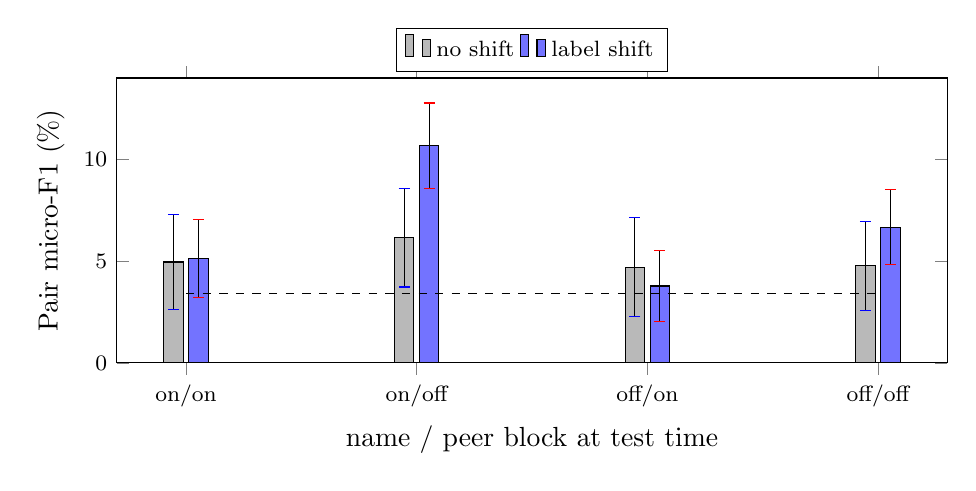
\begin{tikzpicture}
\begin{axis}[ybar,width=\columnwidth,height=5.2cm,bar width=7pt,ymin=0,ymax=14,ylabel={Pair micro-F1 (\%)},
 symbolic x coords={1,2,3,4},xtick=data,xticklabels={on/on,on/off,off/on,off/off},xlabel={name / peer block at test time},
 legend style={at={(0.5,1.02)},anchor=south,legend columns=3,font=\footnotesize},tick label style={font=\footnotesize},
 error bars/y dir=both,error bars/y explicit]
\addplot+[fill=gray!55,draw=black] coordinates {(1,4.96) +- (0,2.35) (2,6.16) +- (0,2.43) (3,4.71) +- (0,2.44) (4,4.77) +- (0,2.19)};
\addplot+[fill=blue!55,draw=black] coordinates {(1,5.14) +- (0,1.91) (2,10.68) +- (0,2.09) (3,3.78) +- (0,1.76) (4,6.67) +- (0,1.84)};
\draw[dashed] (axis cs:1,3.42) -- (axis cs:4,3.42);
\legend{no shift,label shift,trivial floor}
\end{axis}
\end{tikzpicture}
\caption{Who\&When pair micro-F1 of the 14-encoder ensemble by test-time block mask, with and without label shift (bars: 95\% intervals; dashed: trivial floor). Shift helps only when the peer block is hidden.}
\label{fig:ww}
\end{figure}
